\section{Hashing and Membership}
\subsection{Invertible Bloom Lookup Table}
\begin{itemize}
	\item The IBLT data structure $\mathcal B$ is a randomized data structure storing a set of key-value pairs
  \begin{itemize}
  	\item It is designed with respect to a threshold number of key $t$ 
    \item A structure is successful for an operation with high probability is under the assumption that the actual number of keys $n$ in the structure is less that or equal to $t$
  \end{itemize}
	\item It is assumed:
  \begin{itemize}
		\item That keys and values fit in a single word of memory
		\item Each such word can be viewed as an integer, character string, floating-point number, etc.
		\item w.l.o.g. keys and values are viewed as positive integers
  \end{itemize}
  \item Overflow must be considered when taking the sums of the keys and/or values
  \begin{itemize}
  	\item Overflow is with suitable sized memory words overflow never needs to be a consideration
    \item The system supports graceful overflow i.e. $(x+y) -y = x$ even if the sum results in an overflow
    \item XORs can be used instead of sums in many cases
  \end{itemize}
  \item It uses $k$ random hash functions $h_1, \dots, h_k$ 
\end{itemize}

\subsection{Operations}
\begin{itemize}
	\item $\textsc{insert}(x,y)$: insert the key-value pair, $(x,y)$, into $\mathcal B$
  \begin{itemize}
  	\item This operation always succeeds, assuming that all keys are distinct
  \end{itemize}
	\item $\textsc{delete}(x,y)$: delete the key-value pair, $(x,y)$, into $\mathcal B$
  \begin{itemize}
  	\item This operation always succeeds, provided $(x,y) \in \mathcal B$
  \end{itemize}
	\item $\textsc{get}(x)$: return the value $y$ such that there s a key-value pair $(x,y)$ in $\mathcal B$
  \begin{itemize}
		\item If $y = \text{null}$ is returned then $(x,y) \notin \mathcal B$ for any value of $y$
		\item With low (but constant) probability this operation may fail, returning a "not found" error condition, in this case there may or may not be a key-value pair $(x,y)$ in $\mathcal B$
  \end{itemize}
	\item $\textsc{listEntries}()$: list all the key-value pairs being stored in $\mathcal B$
  \begin{itemize}
		\item With low (inverse polynomial in $t$) probability, this operation may return a partial list along with an "list-incomplete" error condition
  \end{itemize}


  \item When IBLT $\mathcal B$ is first created, it initializes a lookup table $T$ of $m$ cells
  \begin{itemize}
	  \item Each of the cells in $T$ stores a constant number of fields, each of which corresponds to a single memory word
  	\item An important feature of the data structure is that at times the number of key-value pairs in $\mathcal B$ can be much larger than $m$
  \end{itemize}
	\item But the space used for $\mathcal B$ remains $O(m)$ words
	\item Each cell contains three field:
  \begin{itemize}
		\item A $\text{count}$ field, which counts the number of entries that have been mapped to this cell
		\item A $\text{keySum}$ field, which is the sum of all the keys that have been mapped to this cell
		\item A $\text{valueSum}$ field, which is the sum of all the values that have been mapped to this cell
  \end{itemize}
  \item $\textsc{insert}(x,y)$:
  \begin{itemize}
    \item \textbf{for} each (distinct) $h_i(x)$, for $i=1, \dots, k$ \textbf{do}
    \begin{itemize}
      \item add $1$ to $T[h_i(x)]$.count
      \item add $x$ to $T[h_i(x)]$.keySum
      \item add $y$ to $T[h_i(x)]$.valueSum
    \end{itemize}
  \end{itemize}

  \item $\textsc{delete}(x,y)$:
  \begin{itemize}
    \item \textbf{for} each (distinct) $h_i(x)$, for $i=1, \dots, k$ \textbf{do}
    \begin{itemize}
      \item subtract $1$ to $T[h_i(x)]$.count
      \item subtract $x$ to $T[h_i(x)]$.keySum
      \item subtract $y$ to $T[h_i(x)]$.valueSum
    \end{itemize}
  \end{itemize}
  \begin{figure}[H]
  	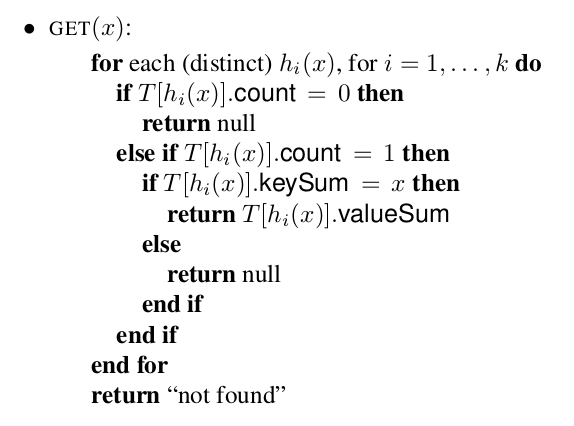
\includegraphics[width=200pt]{img/get}
  \end{figure}
  \item \textbf{Lemma} The GET operation succeeds except with some small probability if $h_1, \dots, h_k$ are truly random hash functions chosen independently at random
  \begin{itemize}
  	\item Let $E_{i,y,j}$ to be the event that $h_i(x) = h_j(y)$
    \item Then $\Pr[E_{i,y,j}] = \frac1m$ since the hash functions are chosen independently at random
    \item Let $E_i$ be the event that there is at least one collision on $h_i(x)$
    \item Then $E_i = \bigcup_{y,j} E_{i,y,j}$ and using the union bound it must be the case that $\Pr[E_i] \leq \frac{nk}m$ 
    \item Thus $\Pr[h_i(x) \text{ no collision}] \geq 1 - \frac{kn}m$
    \item Then the probability that get is answered can be computed as follows
    \begin{align*}
      \Pr[\text{Answer } \textsc{get}] &= 1- \Pr[\land_{i}E_i] \\
                                       &= 1- \prod \Pr[E_i] \text{ (independently chosen)} \\
                                       &\geq 1- \prod \left(\frac{nk}m\right)^k \\
                                       &\geq 1- \prod \left(\frac{tk}m\right)^k \ (n \leq t)
    \end{align*}
    If $m = k \cdot t$ then this probability becomes $1-\left(\frac12\right)^k$ and thus this operation succeeds except with small probability
  \end{itemize}
  \item \textbf{Lemma} When $m = e^2 k t$ then the list operation fails with probability $\leq O(t^{-k+2})$ when $n \leq t$ 
\end{itemize}    

\newpage
%%% Local Variables:
%%% mode: latex
%%% TeX-master: "ra-noter"
%%% End:
